\documentclass[10pt,letterpaper]{scrartcl}
\usepackage{amsfonts,amsmath,amssymb,braket,xcolor,dsfont,enumerate,fontawesome,graphicx}%,hyperref,
\usepackage{listings,multicol,mathtools,textcomp,tikz,pgfplots,wrapfig}
\usepackage[inner=2cm,outer=2cm,top=2cm,bottom=2cm]{geometry}
\usepackage{tabularx}
\usepackage{booktabs}
\usetikzlibrary{arrows}
\pgfplotsset{compat=1.12}

\pagestyle{empty}
\setlength{\parindent}{0pt}
\setlength{\parskip}{6pt}

\newcommand{\dx}{\;\mathrm{d}x}

\begin{document}

\begin{minipage}{.2\textwidth}

\includegraphics[width=42pt]{ubc-logo.png}
\end{minipage}
\hfill
\begin{minipage}{.75\textwidth}
\setlength{\parskip}{6pt}
\begin{flushright}
{\sffamily
\textbf{MATH521}\\
\textbf{Numerical Analysis of Partial Differential Equations}

Winter 2017/18, Term 2\\
Timm Treskatis
}
\end{flushright}
\end{minipage}

\section*{Homework Assignment 6}

Please submit the following files as indicated below: \hfill \faFileCodeO \: source code \hfill \faFilePdfO \: PDF file \hfill \faFilePictureO \: image file \hfill \faFileMovieO \: video file

\paragraph*{Question 1 $\vert$ 2 marks $\vert$ \faFilePdfO}

Given three points $a,b,c \in \mathds{R}^2$ that are not collinear (not all on one line) and that are sorted in anticlockwise order, we define
\begin{align*}
T &= \Delta(a,b,c) \qquad \text{(the triangle with these vertices)}\\
P &= P_2(T)\\
L &= \Set{ p\mapsto p(a), \quad
 p\mapsto p(b),\quad
 p\mapsto p(c),\quad
 p\mapsto \frac{\partial p}{\partial n}\left(\frac{a+b}{2}\right),\quad
 p\mapsto \frac{\partial p}{\partial n}\left(\frac{b+c}{2}\right),\quad
 p\mapsto \frac{\partial p}{\partial n}\left(\frac{c+a}{2}\right)} \subset P^*
\end{align*}

\begin{center}
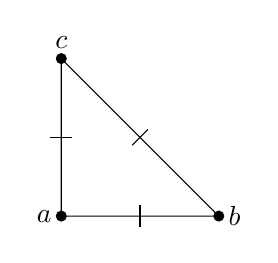
\begin{tikzpicture}
\draw (0,0) node[anchor=east]{$a$}
  -- (2,0) node[anchor=west]{$b$}
  -- (0,2) node[anchor=south]{$c$}
  -- cycle;
\fill (0,0) circle[radius=2pt];
\fill (2,0) circle[radius=2pt];
\fill (0,2) circle[radius=2pt];
\draw (1,-0.14) -- (1,0.14);
\draw (-0.14,1) -- (0.14,1);
\draw (1-0.1,1-0.1) -- (1+0.1,1+0.1);
\end{tikzpicture}
\end{center}

\begin{enumerate}[(a)]
\item Show that prescribed data for
\begin{equation*}
p(a), \quad
 p(b),\quad
 p(c),\quad
 \frac{\partial p}{\partial n}\left(\frac{a+b}{2}\right),\quad
 \frac{\partial p}{\partial n}\left(\frac{b+c}{2}\right)\quad \text{and} \quad
 \frac{\partial p}{\partial n}\left(\frac{c+a}{2}\right)
\end{equation*}
uniquely determines any $p \in P$. You don't have to show that such $p$ always exists.
\newpage

\item Now let $\Omega^h$ be a domain with a regular triangulation $\mathcal{T}^h$ such that
\begin{equation*}
\bar{\Omega}^h = \bigcup_{T\in \mathcal{T}^h} T.
\end{equation*}
Is the space
\begin{equation*}
V^h = \Set{v^h: \bar{\Omega}^h\to \mathds{R} | \left. v^h\right\rvert_T \in P_2(T), v^h \text{ is continuous in all vertices}, \frac{\partial v^h}{\partial n} \text{ is continuous in all edge midpoints} }
\end{equation*}
$H^1$-conforming, i.e. is $V^h \subset H^1(\Omega ^h)$?

\emph{Hint:} Check if there may be any jumps of $v^h$ across triangle edges.
\end{enumerate}
\newpage

\paragraph*{Question 2 $\vert$ 3 marks $\vert$ \faFileCodeO \: \faFilePictureO \: \faFilePdfO}

We will now complete our finite-element solver for the linear elasticity problem
\begin{equation}\label{eq:le}
\begin{aligned}
-c\Delta u + a u &= f &&\text{in } \Omega\\
u &= g && \text{on } \partial\Omega.
\end{aligned}
\end{equation}

\begin{enumerate}[(a)]
\item Remove lines 1-10 from \texttt{discretiseLinearElasticity.m} and uncomment the sections of code that are currently commented out. Complete the missing commands, including the subfunction \texttt{assembleStiffness}. Also inspect the \texttt{assembleLoad} subfunction.
\item Write a script \texttt{hw6.m} which
\begin{itemize}
\item solves the linear elasticity problem on $\Omega^h$, which you may choose from \texttt{kiwi.mat}, \texttt{maple.mat}, \texttt{pi.mat}, \texttt{ubc.mat}. You may also select your own data for $f(x_1,x_2)$, $g(x_1,x_2)$, $a$ and $c$.

\emph{Hint:} You have to set \texttt{GammaD = @(x1,x2) true(size(x1))}. For debugging, you might want to use \texttt{video10.mat} and check the sparsity patterns of the various matrices.
\item calculates the $L^2$, $H^1$ and energy norms
\begin{align*}
\lVert u^h \rVert_{L^2} &= \sqrt{\int\limits_{\Omega^h} \lvert u^h \rvert^2 \dx}\\
\lVert u^h \rVert_{H^1} &= \sqrt{\lVert u^h \rVert_{L^2}^2 + \lVert \nabla u^h \rVert_{L^2}^2} = \sqrt{\int\limits_{\Omega^h} \lvert u^h \rvert^2 \dx + \int\limits_{\Omega^h} \lvert \nabla u^h \rvert^2 \dx}\\
\lVert u^h \rVert_{B} &= \sqrt{B(u^h,u^h)} = \sqrt{c\int\limits_{\Omega^h} \lvert \nabla u^h \rvert^2 \dx + a \int\limits_{\Omega^h} \lvert u^h \rvert^2 \dx}
\end{align*}
of the solution, where $B$ is the bilinear form corresponding to the elliptic operator
\item creates undistorted plots of the mesh, the force $f$ and the solution $u^h$
\end{itemize}
\item What problem do you solve numerically when you set \texttt{GammaD = @(x1,x2) false(size(x1))}? Analyse the code to infer its weak formulation:
\end{enumerate}

\vfill

\paragraph*{Your Learning Progress $\vert$ \faFilePdfO}

What is the one most important thing that you have learnt from this assignment?

\vspace*{3mm}
\hrulefill

\vspace*{3mm}
\hrulefill

Any new discoveries or achievements towards the objectives of your course project?

\vspace*{3mm}
\hrulefill

\vspace*{3mm}
\hrulefill

What is the most substantial new insight that you have gained from this course this week? Any \emph{aha moment}?

\vspace*{3mm}
\hrulefill

\vspace*{3mm}
\hrulefill

\end{document}
